\documentclass{article}
\usepackage{amsmath}
\usepackage[top=-1cm, bottom=2cm, left = 1cm, right = 1cm]{geometry}
\usepackage{graphicx}
\graphicspath{{images/}}
\title{List 1 report}
\author{Albert Kołodziejski}
\begin{document}
\maketitle
\section*{Results:}
\small
\begin{center}
    \begin{tabular}{| c | c | c || c | c | c || c | c | c || c | c | c ||}
        \hline
        data & best & MST & \multicolumn{3}{c||}{Local search based on MST} & \multicolumn{3}{c||}{Local search} & \multicolumn{3}{c||}{Local search speeded up}\\ 
        \cline{4-12}
        name & solution & weight & avg steps & avg cost & min cost & avg steps & avg cost & min cost & avg steps & avg cost & min cost\\
        \hline
        \hline
        XQF131 & 564 & 474 & 32.31 & 602.60 & 579 & 133.72 & 612.46 & 582 & 124.61 & 981.18 & 813\\
        \hline
        XQG237 & 1019  & 897 & 47.16 & 1087.17 & 1064 & 261.54 & 1117.13 & 1066 & 245.06 & 1944.00 & 1523\\
        \hline
        PMA343 & 1368  & 1179 & 76.09 & 1455.45 & 1426 & 404.46 & 1483.75 & 1417 & 395.05 & 2586.37 & 2138\\
        \hline
        PKA379 & 1332 & 1151 & 92.45 & 1408.91 & 1383 & 450.21 & 1447.03 & 1383 & 438.60 & 2534.46 & 2041\\
        \hline
        BCL380 & 1621 & 1444 & 61.65 & 1710.94 & 1675 & 449.25 & 1818.05 & 1726 & 412.20 & 3442.95 & 2754\\
        \hline
        PBL395 & 1281 & 1124 & 75.45 & 1383.25 & 1356 & 459.17 & 1427.61 & 1359 & 426.74 & 2652.45 & 2156\\
        \hline
        PBK411 & 1343 & 1180 & 82.13 & 1436.26 & 1420 & 485.06 & 1492.49 & 1435 & 447.42 & 2829.54 & 2202\\
        \hline
        PBN423 & 1365 & 1201 & 83.63 & 1467.92 & 1438 & 498.31 & 1522.15 & 1445 & 465.91 & 2828.98 & 2325\\
        \hline
        PBM436 & 1443 & 1269 & 93.26 & 1560.06 & 1535 & 513.56 & 1610.40 & 1529 & 473.36 & 3039.58 & 2425\\
        \hline
        XQL662 & 2513 & 2240 & 124.13 & 2694.68 & 2645 & 812.53 & 2813.24 & 2708 & 771.82 & 5270.68 & 4347\\
        \hline
        XIT1083 & 3558 & 3253 & 232.96 & 3841.46 & 3771 & 1386.61 & 4019.99 & 3919 & 1330.18 & 7811.51 & 6595 \\
        \hline
        ICW1483 & 4416 & 4015 & 300.61 & 4761.54 & 4706 & 1930.10 & 4982.06 & 4868 & 1864.24 & 9745.39 & 8407\\
        \hline
        DJC1785 & 6115 & 5541 & 372.50 & 6543.71 & 6459 & 2352.39 & 6881.12 & 6742 & 2285.75 & 13097.22 & 11461\\
        \hline
        DJB2036 & 6197 & 5593 & 398.55 & 6682.48 & 6633 & 2723.75 & 7009.80 & 6852 & 2658.48 & 13797.59 & 11841\\
        \hline
        PDS2566 & 7643 & 6956 & 443.28 & 8178.85 & 8136 & 3481.51 & 8713.09 & 8550 & 3041.39 & 17456.76 & 15112\\
        \hline
    \end{tabular}
    \end{center}
\normalsize
As we can see both local search starting from random permutation, and local search starting from cycle made out of mst resulted in good approximation, with a little advantage for the second one. Speeding up local search resulted in result worse results, it was fast but still required a lot of steps, whereas local search based on mst was fast, required an order of magnitude fewer steps, and had the best results. It is important to pick a good starting point for metaheuristic.
    \section*{QA:}
    \begin{center}
        \textbf{Why with Euclidean metric this algorithm produce a cycle without edges that cross?}
    \end{center}
    \begin{center}
        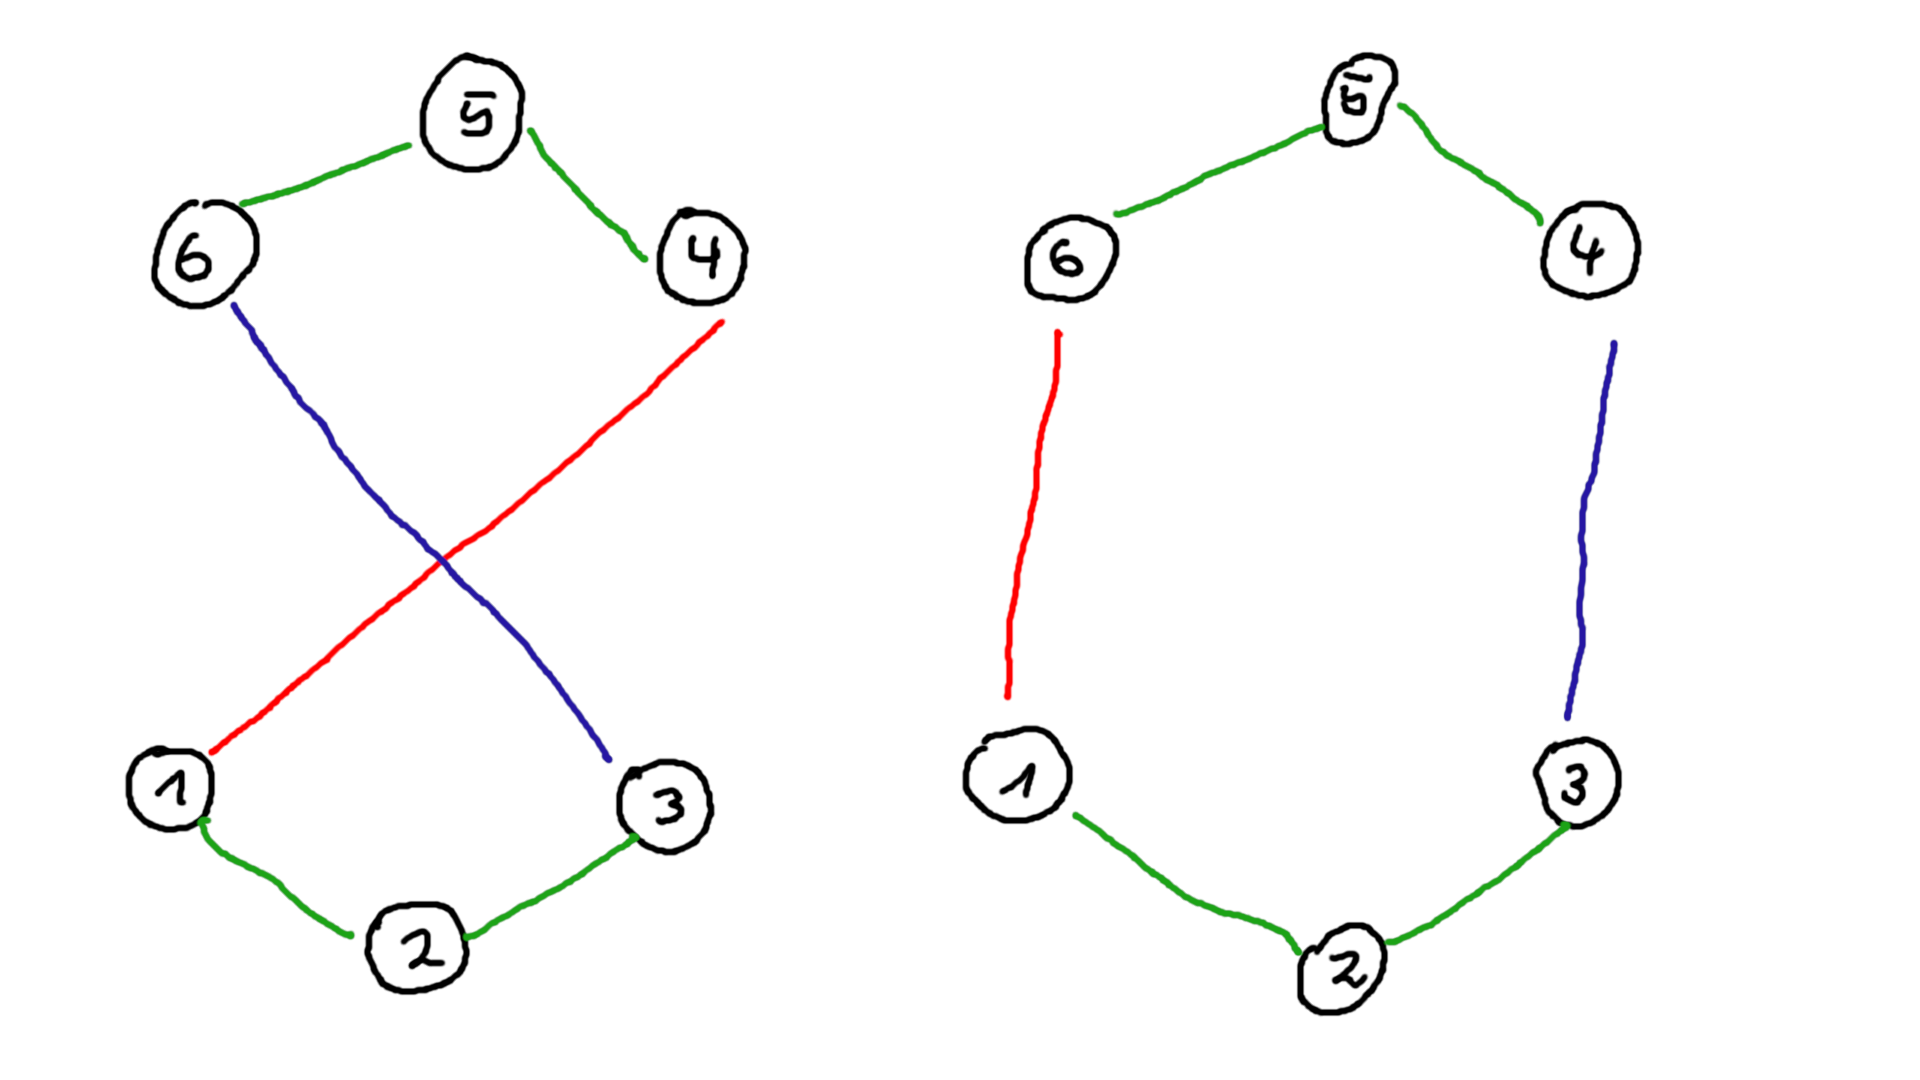
\includegraphics[scale=0.4]{first} 
    \end{center}
    Because inversion is about demangling crosses:
    \[
        \pi = (1, 2, 3, 6, 5, 4)    
    \]
    after \textit{\(invert(\pi, 6, 4)\)}:
    \[
        \pi = (1, 2, 3, 4, 5, 6)    
    \]

    \begin{center}
        \textbf{Why it is not a case in this metric?}
    \end{center}
    \begin{center}
        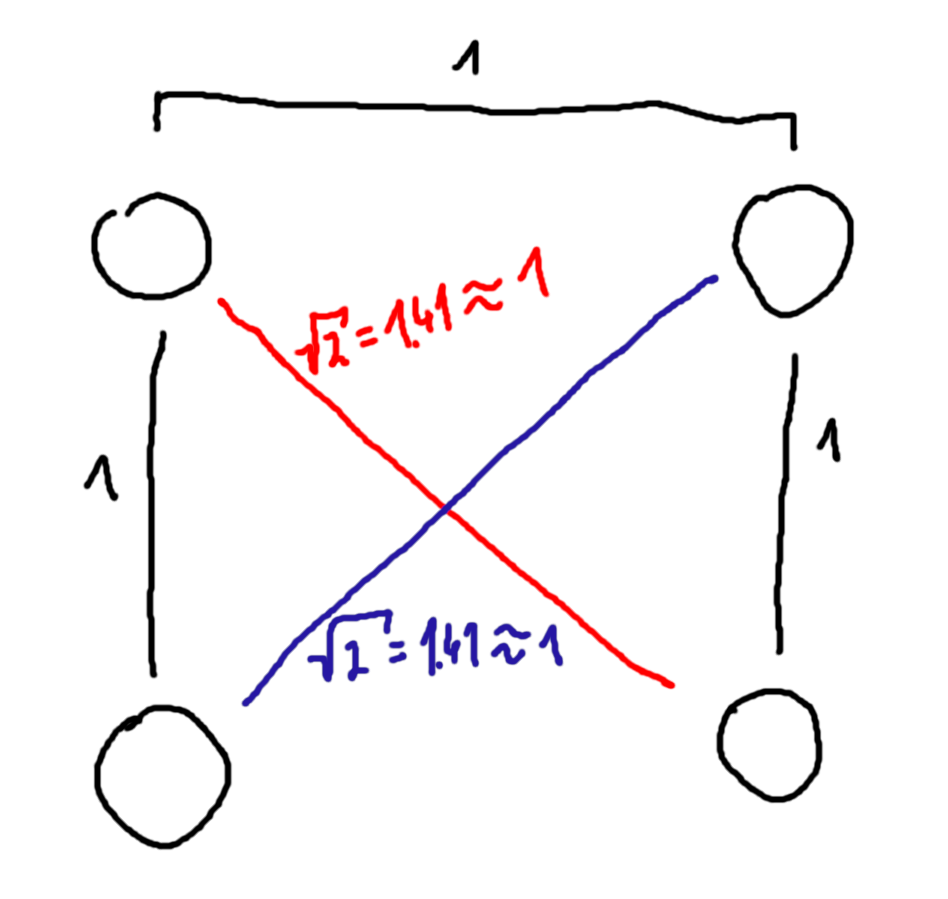
\includegraphics[scale=0.4]{second} 
    \end{center}
    The spite of demangled lines having less length in Euclidean metric, rounded crossed edges have also lengths one and one.
\end{document}